\documentclass{ltjsarticle}
\usepackage{amsmath}
\usepackage{amssymb}
\usepackage{ascmac}
\usepackage[dvipdfmx]{graphicx}
\usepackage[colorlinks=true, allcolors=blue]{hyperref}
\usepackage{fancybox}

\begin{document}

\title{応用数学}
\author{秋葉洋哉}
\maketitle
\section{線形代数}
\subsection{行列}
ある連立方程式が与えられたとき、その連立方程式を行列で表すことができる。例えば、以下の連立方程式を考える。
\begin{align}
 5x_1 + 2x_2 = 10 \\
 3x_1 + 4x_2 = 11
\end{align}
行列は連立方程式の各係数を縦横に並べたものであり、上述した連立方程式は行列を用いて以下のように表される。
\begin{align}
\mathbf{A} \mathbf{x} &= \mathbf{b}\\
\begin{pmatrix}
  5 & 2 \\
  3 & 4
\end{pmatrix}
\begin{pmatrix}
  x_1 \\
  x_2
\end{pmatrix}
&=
\begin{pmatrix}
  10 \\
  11
\end{pmatrix}
\end{align}
この時、$\mathbf{A}$のことを行列と呼ぶ。また、$\mathbf{x}$のことをベクトルと呼ぶ。

\newpage

\subsection{逆行列}
行列$\mathbf{A}$に対して、行列$\mathbf{B}$が存在して以下の式が成り立つとき、行列$\mathbf{B}$を行列$\mathbf{A}$の逆行列と呼ぶ。
\begin{align}
\mathbf{A} \mathbf{B} = \mathbf{B} \mathbf{A} = \mathbf{I}
\end{align}
ただし、$\mathbf{I}$は単位行列である。
逆行列の求め方は、掃き出し法、余因子法、逆行列の公式などがある。
ここで、逆行列の存在しない行列を考える。
連立方程式の解が無く、一組に決まらない場合、逆行列は存在しない。
たとえば、以下の連立方程式を考える。
\begin{align}
  x_1 + 2x_2 = 3 \\
  2x_1 + 4x_2 = 6
\end{align}
行列で表すと以下のようになる。
\begin{align}
\begin{pmatrix}
  1 & 2 \\
  2 & 4
\end{pmatrix}
\begin{pmatrix}
  x_1 \\
  x_2
\end{pmatrix}
&=
\begin{pmatrix}
  3 \\
  6
\end{pmatrix}
\end{align}
この時、行列$\mathbf{A}$の逆行列は存在しない。
このことを端的に表すと、2本のベクトルが同一直線上にある場合、逆行列は存在しないということを示している。
つまり、
\begin{align}
\begin{pmatrix}
  a & b \\
  c & d \\
\end{pmatrix}
=
\begin{pmatrix}
  \vec{v}_1 \\
  \vec{v}_2
\end{pmatrix}
\end{align}
において、二つのベクトルに囲まれる平行四辺形の面積が0の場合、逆行列は存在しないということである。
この「面積」を行列式と呼び、以下のように表す。
\begin{align}
\begin{vmatrix}
  a & b \\
  c & d \\
\end{vmatrix}
=
\begin{vmatrix}
  \vec{v}_1 \\
  \vec{v}_2
\end{vmatrix}
\end{align}
\par
行列式は判別式(determinant)とも呼ぶ。なぜなら、行列式が0の場合、連立方程式の解が一意に定まらないため、解が存在しないということを示すからである。
行列式は、計算上4つの重要な性質を有する。
\begin{enumerate}
\item 同じ行ベクトルが含まれていると行列式はゼロになる。
\item 1つのベクトルが\lambda 倍されると行列式は\lambda 倍される。
\item 他の成分がすべて同じで、i番目のベクトルだけが違った場合、行列式の足し合わせになる。
\item 行を入れ替えると符号が変わる。
\end{enumerate}
行列式の計算方法は、余因子展開、行列の対角成分を用いる方法、行列の固有値を用いる方法などがある。
$2\times2$の行列式の計算方法は、以下のようになる。
\begin{align}
\begin{vmatrix}
  a & b \\
  c & d \\
\end{vmatrix}
= ad - bc
\end{align}
$3\times3$の行列式の計算方法は、以下のようになる。
\begin{align}
\begin{vmatrix}
  a & b & c \\
  d & e & f \\
  g & h & i \\
\end{vmatrix}
= aei + bfg + cdh - ceg - bdi - afh
\end{align}

\newpage

\subsection{固有値と固有ベクトル}
正方行列$\mathbf{A}$に対して、以下の式が成り立つとき、$\lambda$を行列$\mathbf{A}$の固有値、$\mathbf{v}$を行列$\mathbf{A}$の固有ベクトルと呼ぶ。
\begin{align}
\mathbf{A} \mathbf{v} = \lambda \mathbf{v}
\end{align}
固有値と固有ベクトルは、行列$\mathbf{A}$の固有方程式を解くことで求めることができる。
固有方程式は以下のように表される。
\begin{align}
\begin{vmatrix}
  a - \lambda & b \\
  c & d - \lambda \\
\end{vmatrix}
= 0
\end{align}
固有値と固有ベクトルは、行列$\mathbf{A}$の対角化に用いられる。
行列$\mathbf{A}$が対角化可能であるとは、行列$\mathbf{A}$が固有ベクトルを基底とする行列$\mathbf{P}$と対角行列$\mathbf{D}$を用いて以下のように表されることをいう。
\begin{align}
\mathbf{A} = \mathbf{P} \mathbf{D} \mathbf{P}^{-1}
\end{align}
ただし、$\mathbf{P}$は固有ベクトルを列ベクトルとして並べた行列、$\mathbf{D}$は固有値を対角成分に持つ行列である。
\par
固有値と固有ベクトルは、行列の対角化に用いられるだけでなく、主成分分析、特異値分解、クラスタリングなどの機械学習アルゴリズムにも広く用いられる。

\newpage

\subsection{特異値分解}
$\mathbf{A}$が正方行列でない場合、特異値分解という方法で、正方行列と同様に分解することができる。
行列$\mathbf{A}$に対して、以下の式が成り立つとき、$\mathbf{U}$を左特異ベクトル、$\mathbf{V}$を右特異ベクトル、$\mathbf{\Sigma}$を特異値と呼ぶ。
\begin{align}
\mathbf{A} = \mathbf{U} \mathbf{\Sigma} \mathbf{V}^T
\end{align}
特異値の求め方は、以下の通りである。
まず、特異値が存在するには、2つの単位ベクトル$\vec{v}, \vec{u}$が以下の条件を満たす必要がある。
\begin{align}
\mathbf{A} \vec{v} = \sigma \vec{u} \label{v1}\\
\mathbf{A}^T \vec{u} = \sigma \vec{v} \label{v2}
\end{align}
このような特殊な単位ベクトルがある時、特異値分解できる。
ここで、$\sigma$を$\Sigma$とし、行列で表すと、以下のようになる。
\begin{align}
\Sigma = \begin{pmatrix}
  \sigma_1 & 0 & \dots & 0 \\
  0 & \sigma_2 & \dots & 0 \\
  \vdots & \vdots & \ddots & \vdots \\
  0 & 0 & \dots & \sigma_n \\
\end{pmatrix}
\end{align}
さらに、$\vec{v}, \vec{u}$を列ベクトルとして並べた行列を$\mathbf{V}, \mathbf{U}$とし、式\eqref{v1}と式\eqref{v2}を行列で表すと、以下のようになる。
\begin{align}
\mathbf{A} \mathbf{V} &= \mathbf{U} \mathbf{\Sigma} \\
\mathbf{A}^T \mathbf{U} &= \mathbf{V} \mathbf{\Sigma}^T
\end{align}
これらの式を変形すると、
\begin{align}
\mathbf{A} &= \mathbf{U} \mathbf{\Sigma} \mathbf{V}^{-1}\\
\mathbf{A}^T &= \mathbf{V} \mathbf{\Sigma}^T \mathbf{U}^{-1}
\end{align}
となり、これらの積は、
\begin{align}
\mathbf{A} \mathbf{A}^T &= \mathbf{U} \mathbf{\Sigma} \mathbf{V}^{-1} \mathbf{V} \mathbf{\Sigma}^T \mathbf{U}^{-1} = \mathbf{U} \mathbf{\Sigma}^2 \mathbf{U}^{-1}
\end{align}
となる。これより、$\mathbf{A} \mathbf{A}^T$を固有値分解することで、特異ベクトルと特異値の2乗が求められる。
特異値分解は、主成分分析、画像圧縮、レコメンデーションシステムなどに広く用いられる。

\paragraph{1章 参考文献}

\newpage

\section{統計学}
\subsection{集合}
$S$という集合に属する要素を$a$とすると、$a$について以下のように表す。
\begin{align}
a \in S
\end{align}
要素が$a$以外にも、$b, c, d$がある場合、$S$について以下のように表す。
\begin{align}
S = \{a, b, c, d\}
\end{align}
また、集合の内部に$M$という部分集合がある場合、以下のように表す。
\begin{align}
M \subset S
\end{align}
確率・統計に登場する「事象」は、「集合」と同じ概念であると考えることができる。
たとえば、サイコロを振るとき、出る目が「1」である事象を$A$とすると、以下のように表す。
\begin{align}
A = \{1\}
\end{align}
また、サイコロを振るとき、出る目が「偶数」である事象を$B$とすると、以下のように表す。
\begin{align}
B = \{2, 4, 6\}
\end{align}
このように決めておくことで、確率を数式で表すことができる。

\par
和集合・共通部分・絶対補・相対補は記号を用いて以下で表す。
\begin{align}
A \cup B & : A \text{と} B \text{の和集合} \\
A \cap B & : A \text{と} B \text{の共通部分} \\
U \ A = \bar{A} & : A \text{の絶対補} \\
B \ A & : A \text{の相対補}
\end{align}
これらの概念も、確率・統計において重要な役割を果たす。

\subsection{確率}
確率は大きく分けると「頻度確率」と「ベイズ確率」の2つに分類される。
\par
頻度確率は、試行を繰り返し、その結果を観測することで確率を求める方法である。
例えば、10本のくじを引いて当選する確率を調べたところ、100回試行したときに10回当選したという事実から、当選確率は10\%であるという結論を導くことができる。
\par
ベイズ確率は、事前確率と事後確率を用いて確率を求める方法である。
例えば、医者が患者に対して、「あなたは40\%の確率でインフルエンザに感染しています」と診断したとしたとき、その医者は、別の医者100人が同じ診断を行った結果、40人が同様に感染していると診断するだろう、と考えているのではなく、患者の症状や病歴などを考慮して、事前確率を修正することで、事後確率を求める。
\par
頻度確率は客観確率とも呼ばれ、ベイズ確率は主観確率とも呼ばれる。

\par
確率を定義する。
ある事象$A$が起こる確率を$P(A)$とすると、以下のように表す。
\begin{align}
P(A) = \frac{n(A)}{n(U)}
\end{align}
ただし、$n(A)$は事象$A$が起こる回数、$n(U)$は全事象が起こる回数である。

\par
ここで、集合$A$と集合$B$の共通部分の確率を求める。
\begin{align}
  P (A \cup B) &= P (A) P(B|A)
\end{align}
ただし、$P(B|A)$は、条件付き確率と呼ばれる。

\subsection{条件付き確率}
条件付き確率は、ある事象$B$が与えられた下で、別の事象$A$が起こる確率のことであり、
\begin{align}
P(A|B) = \frac{P(A \cap B)}{P(B)}
\end{align}
で表される。  
例えば、雨が降っている条件下で交通事故に遭う確率を求める場合、雨が降っているという事象$B$が起こったときに、雨が降っているかつ交通事故に遭うという事象$A \cap B$が起こる確率を求めることで導出することができる。確率で表しているが、実際には、事象$A \cap B$が起こる回数を事象$B$が起こる回数で割ることで求めることができる。つまり、
\begin{align}
P(A|B) = \frac{n(A \cap B)}{n(B)}
\end{align}
であるといえる。
ただし、お互いの事象が独立である場合、
\begin{align}
P(A|B) = P(A)
\end{align}
であるから、
\begin{align}
P(A \cap B) = P(A) P(B)
\end{align}
となることに注意する。

\newpage

\subsection{ベイズ則}
ベイズ則は、条件付き確率を用いて、事象$A$が起こったときに、事象$B$が起こる確率を求める方法である。
ベイズ則は以下のように表される。
\begin{align}
P(B|A) = \frac{P(A|B)P(B)}{P(A)}
\end{align}
ここで、具体的な数値を用いてベイズ則の例を示す。
例えば、ある病気の検査があり、その検査の結果が陽性であった場合、実際にその病気にかかっている確率を求めることを考える。
\par
病気である、病気でない、検査で陽性、検査で陰性という4つの事象を考え、それぞれの事象を$D, \bar D, T, \bar T$とする。また、以下の情報が与えられているとする。\\
- 病気にかかっている人の割合 : $P(D) = 0.01$ \\
- 病気にかかっている人が検査で陽性となる確率 : $P(T|D) = 0.99$ \\
- 病気にかかっていない人が検査で陽性となる確率 : $P(T|\bar D) = 0.03$ \\
このとき、ベイズ則を用いて実際に病気にかかっている確率を求めることができる。
まず、分子である、病気にかかっている人が検査で陽性となる確率を求める。
\begin{align}
P(T|D)P(D) = 0.99 \times 0.01 = 0.0099
\end{align}
次に、分母である、検査で陽性となる確率を求める。
\begin{align}
P(T) &= P(T|D)P(D) + P(T|\bar D)P(\bar D)\\ 
&= 0.99 \times 0.01 + 0.03 \times 0.99 = 0.0399
\end{align}
最後に、ベイズ則を用いて、病気にかかっている確率を求める。
\begin{align}
P(D|T) &= \frac{P(T|D)P(D)}{P(T)}\\
&= \frac{0.0099}{0.0399} \\
&\approx 0.247
\end{align}
したがって、検査で陽性となった場合、実際に病気にかかっている確率は約24.7\%であるという結論を導くことができる。

\newpage

\subsection{記述統計と推測統計}
統計学は、大きく分けて「記述統計」と「推測統計」の2つに分類される。
\par
記述統計は、データを集計し、要約することで、データの特徴を把握する方法である。
例えば、平均値、中央値、最頻値、分散、標準偏差などがある。
\par
推測統計は、データから得られた結果をもとに、未知の母集団の特性を推測する方法である。
例えば、母集団の平均値、中央値、最頻値、分散、標準偏差などを推測する。
推測統計では、母集団から標本を抽出し、その標本から得られた結果をもとに、母集団の特性を推測することで、未知の母集団の特性を推測することができる。

\newpage

\subsection{記述統計その1 確率変数と確率分布}
確率変数は、ある事象に対して確率を割り当てる変数のことであり、確率分布は、確率変数が取りうる値とその確率の関係を示す関数のことである。
例えば、サイコロを振るとき、出る目を確率変数$X$とし、その確率分布を以下のように表す。
\begin{align}
P(X=1) = \frac{1}{6}\\
P(X=2) = \frac{1}{6}\\
P(X=3) = \frac{1}{6}\\
P(X=4) = \frac{1}{6}\\
P(X=5) = \frac{1}{6}\\
P(X=6) = \frac{1}{6}
\end{align}
このように、確率変数が取りうる値とその確率の関係を示す関数を確率分布と呼ぶ。
\par
確率分布には、ベルヌーイ分布、マルチヌーイ(カテゴリカル)分布、二項分布、正規(ガウス)分布、ポアソン分布、指数分布、ガンマ分布、ベータ分布、ディリクレ分布などが存在する。
\par
\subsubsection*{ベルヌーイ分布}
ベルヌーイ分布は、コイントスを1回行うイメージである。
ひしゃげたコインを投げたとき、表が出る確率を$\mu$、裏が出る確率を$1-\mu$とし(普通のコインなら$\mu=1/2$のはずだ)、$x$を1のとき成功、0の時失敗を表すパラメータとすると、ベルヌーイ分布は以下のように表す。
\begin{align}
P(x|\mu) = \mu^x(1-\mu)^{1-x}
\end{align}
この時、$E[x] = \mu$, $Var(x) = \mu(1-\mu)$である。
\par
\subsubsection*{二項分布}
二項分布は、ベルヌーイ分布のコイントスを複数回行ったときのイメージである。
コインを$n$回投げたとき、表が出る回数を$x$回とすると、二項分布は以下のように表す。
\begin{align}
P(x|\mu, n) = \frac{n!}{x!(n-x)!} \mu^x(1-\mu)^{n-x}
\end{align}
この時、$E[x] = n\mu$, $Var(x) = n\mu(1-\mu)$である。

\par
\subsubsection*{マルチヌーイ(カテゴリカル)分布}
マルチヌーイ(カテゴリカル)分布は、サイコロを振るイメージである。
サイコロを振ったとき、出る目が1の確率を$p_1$、出る目が2の確率を$p_2$、出る目が3の確率を$p_3$、出る目が4の確率を$p_4$、出る目が5の確率を$p_5$、出る目が6の確率を$p_6$とすると、マルチヌーイ(カテゴリカル)分布は以下のように表す。
\begin{align}
P(x|\mu) = \prod_{k=1}^{K} \mu_k^{x_k}
\end{align}

\par
\subsubsection*{正規(ガウス)分布}
正規(ガウス)分布は、ベル型の連続分布であり、多くの自然現象に適用される。
正規(ガウス)分布は以下のように表す。
\begin{align}
P(x|\mu, \sigma^2) = \frac{1}{\sqrt{2\pi\sigma^2}} \exp \left( -\frac{(x-\mu)^2}{2\sigma^2} \right)
\end{align}
正規(ガウス)分布は、真の分布が分からなくても、サンプルが多ければ、中心極限定理により正規分布に近づくという性質がある。

\par 

\subsection{記述統計その2 期待値}
事象を$X_1, X_2, \dots X_n$ とし、それぞれの確率を$p(X_1), p(X_2), \dots p(X_n)$、確率変数の値を $f(X_1), f(X_2), \dots f(X_n)$とすると、期待値は以下のように表す。
\begin{align}
E[f(X)] = \sum_{k=1}^{n} p(X=x_k) f(X=x_k) \\
E[f(X)] = \int p(X=x) f(X=x) dX
\end{align}

\newpage

\subsection{記述統計その3 分散}
分散は、確率変数の散らばり具合を示す指標であり、以下のように表す。
\begin{align}
Var(X) &= E[(f_{(X=x)} - E_{(f)})^2]\\
&= \text{(二乗の平均)-(平均の二乗) }\\
&= E[X^2] - E[X]^2 
\end{align}
共分散は、2つの確率変数の関係性を示す指標であり、以下のように表す。
\begin{align}
Cov(X, Y) &= E[(f_{(X=x)} - E_{(f)})(g_{(Y=y)} - E_{(g)})]\\
&= E[XY] - E[X]E[Y]
\end{align}
分散を見ることで、平均値からのばらつき具合を知ることができ、共分散を見ることで、2つの確率変数の関係性を知ることができる。例えば、fとgの動き方が似ている時、共分散は正の値を取り、fとgの動き方が逆の時、共分散は負の値を取る。
\par
分散では、元のデータの単位が2乗されるため、元のデータと同じ単位で表すためには、標準偏差を用いる。
標準偏差は、分散の平方根であり、以下のように表す。
\begin{align}
 \sigma(X) = \sqrt{Var(X)}
\end{align}

\newpage

\subsection{推測統計その1 推定}
推測統計では、推定と検定の2つの方法がある。
中でも推定は、母集団の特性を推測する方法であり、大きく分けて「点推定」と「区間推定」の2つに分類される。
\par
点推定は、母集団の特性を1つの数値で推定する方法であり、平均値、中央値、最頻値などを求める推定方法である。
区間推定は、母集団の特性を区間で推定する方法であり、信頼区間、予測区間などを求める推定方法である。
ここでは、点推定で求められた推定値の例として標本平均(母集団から取り出した標本の平均値)の特性を挙げる。
\begin{enumerate}
  \item 一致性:サンプルサイズが大きくなれば、標本平均は母平均に近づく。
  \item 不偏性:サンプル数がいくらであっても、その期待値は母集団の値と同様である。
\end{enumerate}
\par
推定の際には、推定量と推定値の違いを理解することが重要である。
推定量は、パラメータを推定するために利用する数値の計算方法や計算式のことであり、推定値は、推定量を用いて計算された具体的な数値のことである。
例えば、2次関数を微分して出た導関数は推定量であり、傾きは推定値である。

\begin{itembox}[l]{サンプルサイズとサンプル数}
  何度標本の抽出を行ったか、という回数をサンプル数と呼び、1回の抽出で何個体を調べたか、という数をサンプルサイズと呼ぶ。
  例えば、各都道府県から無作為に1000人を抽出して平均身長を算出したとき、サンプル数は47、サンプルサイズは1000となる。 
\end{itembox}

\newpage

\subsection{推測統計その2 標本分散}
標本分散は、母集団の分散を推定するために用いられる統計量であり、以下のように表す。
\begin{align}
\sigma^2 = \frac{1}{n} \sum_{i=1}^{n} (X_i - \bar{X})^2
\end{align}
ここで、$\sigma^2$は標本分散、$n$はサンプルサイズ、$X_i$は各データ、$\bar{X}$は標本平均である。
標本分散は、一致性を満たす一方で、不偏性を満たさない。
これは、たくさんのデータのばらつき具合と、少数のデータのばらつき具合を考えた時、少数のデータのばらつきの方が小さくなると考えることができるためである。

母集団の分散を推定する際には、不偏分散を用いることが多い。
不偏分散は、標本分散をサンプルサイズで補正したものであり、以下のように表す。
\begin{align}
s^2 = \frac{1}{n-1} \sum_{i=1}^{n} (X_i - \bar{X})^2
\end{align}
ここで、$s^2$は不偏分散である。


\newpage

\section{情報科学}
\subsection{導入}
情報の量とは何だろうか。
抽象的な情報量という概念を具体的に表すために、以下の例を考えてみる。
\begin{figure}[htbp]
  \centering
  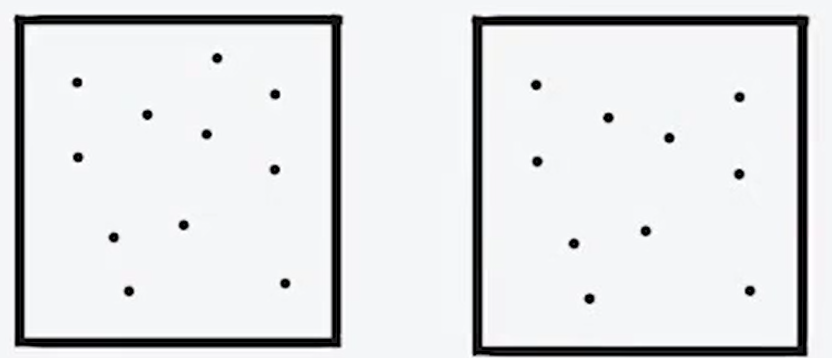
\includegraphics[width=10cm]{box_10.png}
  \caption{箱の中の点の増分 1}
  \label{fig:box_10}
\end{figure}
左の箱には11個の点があり、右の箱には10個の点がある。この差分は1個である。
同様に以下の図をみてみる。
\begin{figure}[htbp]
  \centering
  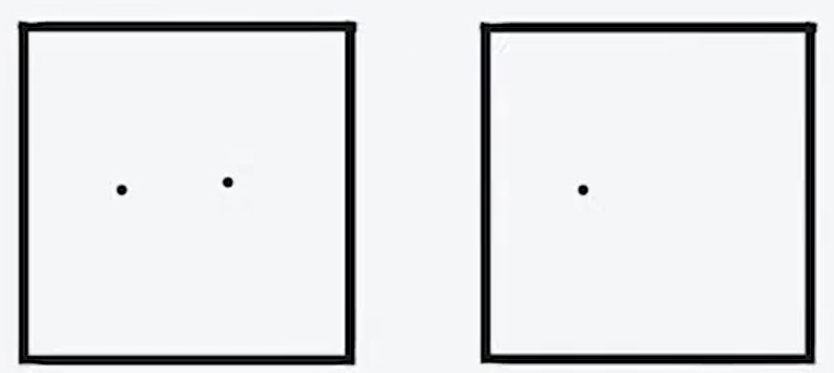
\includegraphics[width=10cm]{box_1.png}
  \caption{箱の中の点の増分 2}
  \label{fig:box_1}
\end{figure}
左の箱には2個の点があり、右の箱には1個の点がある。この差分は1個である。
図\ref{fig:box_10}と図\ref{fig:box_1}を比較すると、どちらも差分が1個だが、明らかに2個から1個になった場合の方が、情報の増え方が大きく感じる。
この経験則から、$w$を変化後の点の数、$\delta w$を変化前との点の差分とすると、情報の増え方を表す指標として、以下の「比率」を考えることができる。
\begin{align}
  \frac{\delta w_1}{w_1} = \frac{1}{10} \\
  \frac{\delta w_2}{w_2} = \frac{1}{1}
\end{align}
この比率は、情報の増え方を表すものであるから、この式を積分することで、情報量を表す指標を導出することができる。
\begin{align}
  \int \frac{1}{w} dw = \log w
\end{align}
\par
この時、$w$は事象の数であるため、確率$p$に置き換えると、以下のように表すことができる。
\begin{align}
  I(p) = - \log p
\end{align}
この式は、「自己情報量」と呼ばれる。
対数の底が2のとき、単位はビット(bit)となり、底がネイピア数のとき、単位はナット(nat)となる。
この式は、情報の珍しさ (=確率の小ささ) を定量化したものであり、確率が小さいほど、情報量が大きくなることを示している。

\subsection{シャノンエントロピー}
自己情報量の期待値を取ることで、シャノンエントロピー(単純にエントロピーともいう)を定義することができる。
\begin{align}
  H(x) &= E(I(x))\\
   &= -E(log(P(x))) \quad\text{(log(P(x))が確率変数になる)}\\
   &= - \sum p(x) \log p(x) \quad\text{(期待値は、確率×確率変数の総和)}
\end{align}
シャノンエントロピーは、新しく得られる情報の量を表す指標と考えることができる。
例えば、表が出る確率が0.99の極端にひしゃげたコインのコイントスを行う場合、そのコインを投げた時に新しく得られる情報の量 (つまり裏が出る事象数) はとても小さく、シャノンエントロピーも小さな値となる。このことを図\ref{fig:coin_shanon}で確認するには、x軸が1.0付近のy軸の値を読み取ればよい。
他に、例えば表が出る確率が0.25, 裏が出る確率を0.75とすると、シャノンエントロピーは
\begin{align}
  -0.25 \log 0.25 - 0.75 \log 0.75 \approx 0.811
\end{align}
となる。
\begin{figure}[htbp]
  \centering
  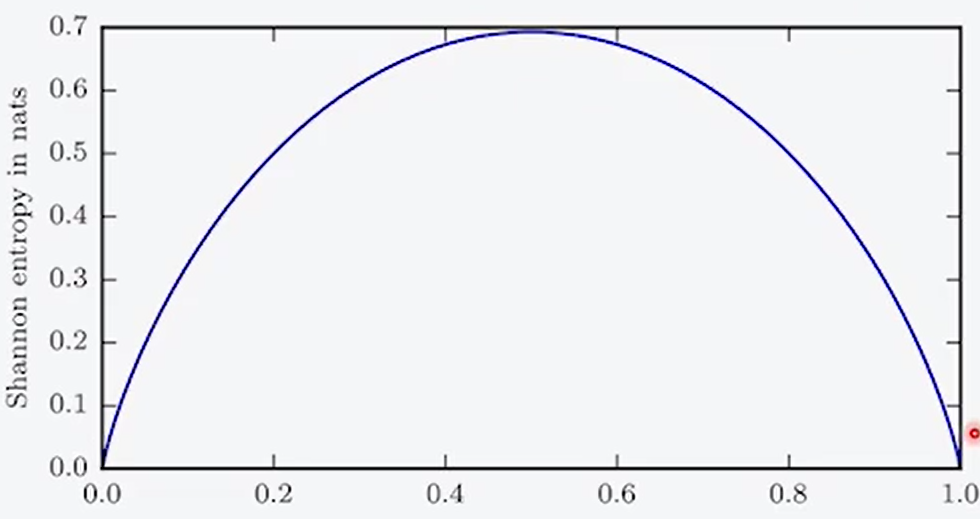
\includegraphics[width=10cm]{coin_shanon.png}
  \caption{ひしゃげたコインのコイントスを行う場合のシャノンエントロピー}
  \label{fig:coin_shanon}
\end{figure}

\subsection{相互情報量}
以下では細工されたサイコロの出る目の確率分布表を示す。
\begin{figure}[htbp]
  \centering
  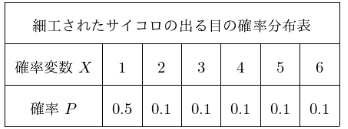
\includegraphics[width=10cm]{./entropy.png}
  \caption{細工されたサイコロの出る目の確率分布}
  \label{fig:dise_entropy}
\end{figure}
このサイコロは、1が出る確率が0.5, それ以外が出る確率が0.1となるような細工がされている。このサイコロを振った時、例えば4の目が出た時に得られる情報量は、$-\log_{2} 0.1$である。また、サイコロを振り出た目を表す確率変数を$X_1$とすると、エントロピー$H(X_1)$は、$-0.5\log_{2}(0.5) - 0.1\log_{2}(0.1) * 5$で表される。

次にもう一度サイコロを振り、出た目を表す確率変数を$X_2$とする。$X_1 = X_2$のとき1, $X_1 \neq X_2$のとき0となる確率変数$Y$を定義する。この時、2つのエントロピー$H(X_1)$と$H(Y)$の和はどのような値をとるだろうか。
この値は結合エントロピーで表される。結合エントロピーは、2つの確率変数のエントロピーの和で定義される。
\begin{align}
  H(X, Y) &= - \sum_{x} \sum_{y} p(x, y) \log p(x, y)\\
\end{align}
表\ref{table:matrix}を参照にすると、上記のサイコロの例での$X_1$と$Y$の結合エントロピー$H(X_1, Y)$は以下のように表すことができる。
\iffalse
\begin{align}
  H(X_1, Y) &= -0.5*0.5\log_{2}(0.5*0.5) - 0.5*0.1\log_{2}(0.5*0.1)*5 - 0.5*0.1\log_{2}(0.5*0.1)*5\\ 
  &- 0.1*0.1\log_{2}(0.1*0.1)*25\\
  &= -0.25\log_{2}(0.25) - 0.05\log_{2}(0.05)*5 - 0.05\log_{2}(0.05)*5 - 0.01\log_{2}(0.01) * 25\\
  &= -0.25\log_{2}(0.25) - 0.5\log_{2}(0.05) - 0.25\log_{2}(0.01)\\
\end{align}
\fi

\begin{table}[htbp]
  \centering
  \caption{結合エントロピーの計算}
  \begin{tabular}{|c|c|c|c|c|c|} \hline
     & $Y$=0 & Y=1 \\ \hline
    $X$=1 & 0.5*0.1*5 & 0.5*0.1 \\ \hline
    $X$=2 & 0.1-0.1*0.1 & 0.1*0.1 \\ \hline
    $X$=3 & 0.1-0.1*0.1 & 0.1*0.1 \\ \hline
    $X$=4 & 0.1-0.1*0.1 & 0.1*0.1 \\ \hline
    $X$=5 & 0.1-0.1*0.1 & 0.1*0.1 \\ \hline
    $X$=6 & 0.1-0.1*0.1 & 0.1*0.1 \\ \hline
  \end{tabular}
  \label{table:matrix}
\end{table}


次に条件付きエントロピーを導入する。条件付きエントロピーは、ある確率変数が与えられたときのエントロピーであり、以下のように表すことができる。
\begin{align}
  H(X|Y) = - \sum_{x} \sum_{y} p(x, y) \log \frac{p(x, y)}{p(y)}
\end{align}
この式は、$X$が与えられたときの$Y$のエントロピーを表す。

相互情報量は、もともとのエントロピー$H(X)$と条件付きエントロピー$H(X|Y)$の差であるため、上記サイコロの例における相互情報量を計算すると、以下のように表すことができる。
\begin{align}
  I(X_1; Y) &= H(X_1) - H(X_1, Y) \\
\end{align}

\if0
相互情報量$I(A;B)$は、もともとのエントロピー$H(X), H(Y)$と結合エントロピー$H(X, Y)$の差であるため、上記サイコロの例における相互情報量を計算すると、以下のように表すことができる。
\begin{align}
  I(X; Y) &= H(X) + H(Y) - H(X, Y) \\
  &= -0.5\log_{2}(0.5) - 0.1\log_{2}(0.1) * 5 -( -\frac{1}{12}\log_{2} \frac{1}{12} - \frac{1}{60}\log_{2} \frac{1}{60} * 5 - \frac{5}{12}\log_{2} \frac{5}{12} - \frac{5}{60}\log_{2} \frac{5}{60} * 5)\\
  &= -0.5\log_{2}(0.5) - 0.1\log_{2}(0.1) * 5 - ( -\frac{1}{12}\log_{2} \frac{1}{12} * 6 - \frac{5}{60}\log_{2} \frac{1}{60} - \frac{5}{12}\log_{2} \frac{5}{12} )
\end{align}

\begin{table}[htbp]
  \centering
  \caption{相互情報量の計算}
  \begin{tabular}{|c|c|c|c|c|c|} \hline
     & X=1 & X=2, 3, 4, 5, 6 \\ \hline
    Y=1 & 1/2*1/6 & 1/10*1/6 \\ \hline
    Y=0 & 1/2*5/6 & 1/10*5/6 \\ \hline
  \end{tabular}
\end{table}
\fi


\newpage

\subsection{カルバック・ライブラーダイバージェンス}
カルバック・ライブラーダイバージェンスは、2つの確率分布の違いを表す指標であり、$Q(x)$を最初に見積もった確率、$P(x)$を真の確率とすると、以下のように表す。
\begin{align}
  D_{KL}(P||Q) &= \mathbb{E}_{x \sim P} [ \log \frac{P(x)}{Q(x)}] \\
  &= \mathbb{E}_{x \sim P} [\log P(x) - \log Q(x)] 
\end{align}
ただし、$\mathbb{E}$は引数$[\log P(x)/Q(x)]$を平均したものを表す。
この引数部分を自己情報量を用いて変形すると、以下のように表すことができる。
\begin{align}
  \log P(x)/Q(x) = I(Q(x)) - I(P(x))
\end{align}
$I(Q(x))$が最初に分かっていた情報量、$I(P(x))$が新しく得られた情報量であるため、カルバック・ライブラーダイバージェンスは、$Q$という状態から$P$という状態に変化したときに、どのくらい新しい情報が得られたかを表す指標であるといえる。ただし、$Q$から$P$に変化した場合と、$P$から$Q$に変化した場合で、カルバック・ライブラーダイバージェンスの値は異なり、距離とは異なることに注意する。
カルバック・ライブラーダイバージェンスは、以下で変形することができる。
\begin{align}
  D_{KL}(P||Q) &= \sum P(x)(\log P(x) -\log Q(x)) \\
&= \sum P(x) \log \frac{P(x)}{Q(x)}
\end{align}



\newpage

\subsection{交差エントロピー}
KLダイバージェンスの一部分を取り出したものが交差エントロピーである。
Qについての自己情報量をPの分布で平均している。
\begin{align}
  H(P, Q) &= - \sum P(x) \log Q(x) \\
  &= - \sum P(x) \log \frac{Q(x)}{P(x)} + \sum P(x) \log P(x) \\
  &= D_{KL}(P||Q) + H(P)
  &= - \mathbb{E}_{x \sim P} [\log Q(x)]
\end{align}
交差エントロピーは分類問題における誤差関数としてよく用いられ、真の確率分布($P(x)$)と推定した確率分布($Q(x)$)に対して、2つの確率分布の誤差を定量的に求めるために使われる。


\paragraph{2章 参考文献}
\begin{enumerate}
  \item 病気に罹患している確率は? ベイズの定理で求める方法を解説『Pythonで動かして学ぶ!』シリーズ (https://codezine.jp/article/detail/14581)
  \item うさぎでもわかる情報量・エントロピー・相互情報量(情報理論)(https://www.momoyama-usagi.com/entry/info-entropy)
\end{enumerate}

\newpage

\end{document}